\documentclass[conference]{IEEEtran}
\usepackage{cite}
\usepackage{amsmath,amssymb}
\usepackage{graphicx}
\usepackage{booktabs}
\usepackage{array}
\usepackage{url}
\begin{document}
\title{Improving Retrospective Fire-Hotspot Models: Regularisation, Nonlinear Features, and Calibration on Observed California Data}
\author{\IEEEauthorblockN{Ayush Singh}\IEEEauthorblockA{Department of Computational Intelligence\\SRM Institute of Science and Technology\\Kattankulathur, India\\as5790@srmist.edu.in}
\and\IEEEauthorblockN{Sarvadnya Kulkarni}\IEEEauthorblockA{Department of Computational Intelligence\\SRM Institute of Science and Technology\\Kattankulathur, India\\ss9878@srmist.edu.in}}
\maketitle
\begin{abstract}
We investigate whether changes to feature transformations, coefficient constraints, class handling, and probability calibration improve retrospective hotspot-occurrence models for California. The experiment uses observed ERA5, VIIRS, MODIS and SRTM inputs on a $0.25^\circ$ grid. Sixty-one candidate configurations are trained on 2021, ranked by average precision on designated 2022 days, and calibrated on separate 2022 days. The selected XGBoost achieves average precision 0.2860, AUC-ROC 0.859 and Brier score 0.01849 on the previously examined 2023 benchmark. Its highest-scored decile captures 60.0\% of positive cell-days, with precision 13.39\%. Matched penalised fits make directional constraints directly comparable; nonlinear and transformed-history alternatives test restrictions of the original formula. Full-population moving-block bootstrap intervals assess sensitivity to temporal dependence. Because 2023 informed the motivation for this follow-up, these results describe retrospective model development, not independent confirmation of generalisation or prospective ignition prediction.
\end{abstract}
\begin{IEEEkeywords}
Wildfire, active fire, hotspot occurrence, ERA5, VIIRS, MODIS, SRTM, calibration.
\end{IEEEkeywords}


\section{Introduction}
An interpretable fire model is useful only if its simplifications survive comparison with simpler explanations of the observations. Satellite hotspot labels are especially demanding in this respect: an ongoing fire can contribute detections on many days, so recent activity alone may rank the response well~\cite{schroeder}. Weather and fuel conditions remain relevant, but a high score does not identify a new ignition or demonstrate advance warning skill.

Our preceding observed-data experiment exposed three opportunities for improvement. A standardized logistic regression outperformed a min--max-scaled additive fit despite using the same nine drivers. A constrained additive fit had higher average precision than its unconstrained alternative, although selection by AUC chose the latter. Finally, tree ensembles and a persistence comparator exceeded the selected additive model. These findings motivated a follow-up focused on the fitting procedure rather than a stronger interpretation of the same coefficients.

Physical reasoning suggests heat, dryness, vegetation, terrain and recent activity as candidate predictors~\cite{jones,wooster}. It does not specify the appropriate statistical penalty, probability calibration, or decision threshold. Nor does it establish that each transformed driver must have a positive conditional coefficient. We therefore ask whether matched regularisation, nonlinear additive effects, less extreme history scaling, and alternative class handling improve performance under a declared validation rule.

This study makes three practical contributions. It compares sign constraints at equal penalties and scales; it evaluates a bounded set of alternatives to a rigid multiplicative index; and it separates selection of the ranking model from selection of its probability mapping. The search includes negative results rather than reporting only the best model. It is explicitly a development study: the 2023 benchmark had already been inspected before these changes were proposed. Validation-only selection reduces direct tuning on that benchmark, but cannot make it an untouched test set again.
\section{Data and Study Design}
\subsection{Sources and spatial unit}
The study covers 1 January 2021 through 31 December 2023. ERA5 single-level hourly reanalysis supplies 2-m temperature, 2-m dewpoint, both 10-m wind components, and volumetric soil water in the 0--7 cm layer~\cite{era5}. Regional ERA5 tiles were read from the public Earthmover archive~\cite{earthmover}; a sampled grid-point hour in each of two months was compared with direct Copernicus downloads. NASA FIRMS standard-processing VIIRS S-NPP 375-m detections provide the response, FRP, and prior hotspot counts~\cite{firms,schroeder}. We retain presumed vegetation fires (type 0) at nominal or high confidence. NASA MOD13A2.061 supplies 1-km, 16-day NDVI and near/mid-infrared reflectances~\cite{modis}. SRTM elevation tiles yield static slope~\cite{srtm}. All raw sources and acquisition metadata are kept with the reproducible code package.

The working bounding box is $32$--$42^\circ$N and $124$--$114^\circ$W. We use only $0.25^\circ$ cell centres inside the US Census California boundary, giving 660 cells. A positive cell-day has at least one retained VIIRS detection. Multiple detections in the same cell-day count as one positive label. This is an observational detection target: cloud, smoke, overpass time, and sensor sensitivity can cause missed activity, while a continuing fire can contribute positives on successive days.

\subsection{Temporal alignment and feature construction}
ERA5 hours are aggregated by UTC day. We use maximum 2-m temperature, wind speed maximum, mean surface soil moisture, and relative humidity computed from temperature and dewpoint at the hour of the daily temperature maximum. The stored feature name \texttt{rh\_min} is a legacy name for this last quantity; it is not the minimum over all 24 hourly humidity estimates. MODIS NDWI is $(\mathrm{NIR}-\mathrm{MIR})/(\mathrm{NIR}+\mathrm{MIR})$. A 16-day composite is made available only after its full window and carried forward until the next available composite; no later composite is interpolated backward. SRTM pixel slopes are averaged within grid cells. Current-day FRP and counts are excluded from predictors; their histories use only days $t-1$ through $t-7$ with weight $0.5^k$ at lag $k$.

Each continuous driver is min--max scaled using only 2021 values, clipped to $[0,1]$ in later years, and then held fixed. Cells with missing MODIS indices are omitted. These rules prevent test-year information from entering the feature scaling or satellite composites. They do not make the study prospective because the same-day ERA5 aggregates are known only after the day.

\subsection{Observation support and missingness}
The spatial mask applies to grid-cell centres. Consequently, a retained coastal or border cell may include water or land outside the state; detections are assigned to the entire cell. The response should be interpreted at that spatial support. MODIS indices are nearest-neighbour samples at grid locations, whereas terrain slopes are cell means. These operations preserve different kinds of spatial variation. In particular, a sampled vegetation pixel need not represent every fuel type within a coarse cell.

Annual source-label totals and model-ready totals have different denominators. The source grid contains 5,376 positive cell-days in 2023, while complete model inputs retain 5,360. Metrics use only the latter rows. Omitting missing vegetation observations may change the evaluated population if missingness is associated with land cover or observation conditions. The current analysis does not estimate that selection effect. Likewise, delaying a composite by its window length prevents use of an unfinished window, but does not reproduce an operational product's actual publication latency.


\section{Candidate Models and Selection}
\subsection{Matched objective and transformed histories}
Let $x_i$ contain nine scaled drivers and $y_i$ the binary hotspot label. Both constrained and unconstrained linear models minimise
\begin{equation}
\begin{aligned}
 \mathcal L(w,b)&=\frac1n\sum_{i=1}^{n}\left[\log(1+e^{z_i})-y_i z_i\right]\\
 &\quad+\frac{\lVert w\rVert_2^2}{2Cn},\qquad z_i=b+x_i^\top w.
\end{aligned}
\end{equation}
The intercept is unpenalised. The constrained version adds $w_j\geq0$; the free version does not. Both use the same numerical optimiser, convergence tolerances and training rows. Values $C\in\{0.01,0.1,1,10,100\}$ are crossed with the two sign conditions and three representations, giving 30 candidates. The representations are min--max drivers, standardized drivers, and standardized drivers after transforming each normalized fire-history input $h$ as $\log(1+1000h)$. The constant 1000 is fixed before the search. It is a feature transformation, not a physical conversion of FRP units.

Training histories are highly concentrated near zero, with occasional large values. Log compression reduces the leverage of extreme observations and gives the linear logit more resolution among small positive histories. It may help ranking, but can also discard useful differences among large fires. Standardisation parameters are fitted on 2021 only. The comparison holds raw information fixed while changing how a penalised linear model can use it.

\subsection{Nonlinear and multiplicative alternatives}
A spline additive logit replaces each linear term with a cubic B-spline expansion:
\begin{equation}
 \operatorname{logit}(p_i)=b+\sum_{j=1}^{9}\sum_k \beta_{jk}B_{jk}(x_{ij}).
\end{equation}
Four training-quantile knots are used per driver, the redundant bias basis is omitted, basis columns are standardized on training rows, and all basis coefficients receive the same $L_2$ penalty. This model permits nonmonotonic marginal responses while remaining additive on the log-odds scale. It does not estimate arbitrary interactions. A separate interaction model augments the log-history representation with temperature--atmospheric-dryness, vegetation--canopy-dryness, atmospheric--soil-dryness, and wind--slope products. Each family uses $C\in\{0.01,0.1,1,10\}$, adding eight candidates.

To examine the zero-gating behaviour of the original product, five further candidates use
\begin{align}
 D_i&=0.3x_{{\rm canopy},i}+0.4x_{{\rm air},i}+0.3x_{{\rm soil},i},\\
 R_i(\epsilon)&=(\epsilon+\tilde T_i)(\epsilon+\widetilde{\rm NDVI}_i)
 (\epsilon+D_i)\notag\\
 &\quad\cdot(1+0.6\tilde U_i+0.4\tilde\theta_i)
 +0.6\widetilde{\rm FRP}_i+0.4\widetilde{\rm Count}_i.
\end{align}
Here $\epsilon\in\{0,0.05,0.2,0.5,1\}$ and the final standardized scalar receives a logistic mapping with $C=100$. Positive offsets reduce suppression when a factor is close to its training minimum. They also change the relative scale of environmental and history terms, so this is a sensitivity family rather than a pure test of one interaction. The five original weights are held fixed at the preceding validation-selected configuration; they are not jointly reoptimised here.

\subsection{Tree ensembles and class handling}
Random Forest, XGBoost and LightGBM each use depths 4 and 8 with three class-handling choices: the original class distribution, inverse-frequency weighting, or training-only SMOTE followed by random undersampling. SMOTE raises the minority/majority ratio to 0.10, then undersampling raises it to 0.30. Unlike the preceding boosted baselines, the resampled candidates do not also apply class weighting. This avoids conflating those two interventions. All use the log-history representation.

Random Forest uses 250 trees and a minimum leaf size of 10. The boosted models use 300 trees, learning rate 0.05 and an $L_2$ parameter of 5. XGBoost uses a minimum child weight of 10, row fraction 0.8 and feature fraction 0.9. LightGBM uses at most 31 leaves and minimum child size 40. Seeds are fixed at 42. These 18 candidates complete a 61-configuration search. The grid is deliberately finite; its winner is not asserted to be globally optimal.

\subsection{Selection and calibration partitions}
All candidate fits use 2021. Within each month of 2022, days 1--14 form the selection set and days 22 through month-end form the calibration set; days 15--21 are excluded from both. This gives 110,448 selection rows and 74,296 calibration rows while representing seasons in both subsets. There is no additional purge at month boundaries, and adjacent dates can remain dependent. The partitions are disjoint in labels but are not independent seasonal trials.

Candidates are ranked by selection average precision (AP), breaking ties by AUC-ROC. AP emphasises retrieval of the rare positive class. The best candidate within each family is retained for reporting, and the overall winner is frozen before the 2023 predictions are scored. No refit on 2022 labels is performed for the ranking model.

Probability mapping is a separate step. Days 22--25 fit three alternatives: identity, a sigmoid fitted to clipped prediction logits, and isotonic regression. The remaining calibration days assess Brier score. The selected mapping is then refitted on all calibration rows. This procedure uses no 2023 labels, although it has limited calibration data and shares the same year's conditions as model selection. Isotonic mapping can introduce score ties and therefore change AP and AUC; both raw and mapped metrics are saved. A sigmoid with nonpositive slope is excluded.

\section{Retrospective Evaluation}
AP is compared with the observed event fraction of 0.02233. We report AUC-ROC, Brier score, and capture at an exactly 10\% row budget rounded upward. Ties at that budget are broken by stable dataset order, so boundary ties can affect the capture count. Brier skill uses the constant probability equal to the original model-ready 2021 rate as its reference. These quantities answer different questions: ranking across thresholds, probability accuracy, and concentration at a specified monitoring budget.

The comparison includes saved predictions from the preceding additive, standardized logistic, persistence and Random Forest models on exactly the same rows. Their training and calibration procedures differ from the new candidates. Gains over them therefore describe whole-pipeline changes and cannot be attributed solely to one architectural change. The matched candidate comparisons provide the narrower evidence about penalties, signs and class handling.

For uncertainty, we use paired circular moving-block resampling of the 365 benchmark days, with block lengths 7 and 30 and 300 replicates per length. Each replicate draws starting days, includes consecutive days modulo the year, and truncates the concatenation to 365 days. All cell-days are retained through day multiplicities; there is no negative-class subsampling. All models receive the same replicate weights. Percentiles of the paired AUC and AP differences form the intervals. Circular wrapping, fixed block lengths and a single observed year remain limitations; the intervals do not account for candidate-selection uncertainty or demonstrate regional transfer.

\section{Results}
\subsection{Selected model and complete comparison}
The validation rule selects XGBoost, with selection AP 0.2375. Its selected probability mapping is identity. The selected configuration uses 300 trees, depth 4, log-compressed histories and the original class distribution. Its complete specification is saved with the model artifact. Table~\ref{tab:results} reports each family winner and the original comparators; bold type identifies the validation-selected model, not whichever row happens to score highest on 2023.

On the retrospective benchmark, the selected model obtains AUC 0.859, AP 0.2860 and Brier score 0.01849. Its mean probability is 0.0224 against observed frequency 0.02233, with Brier skill 0.154 relative to the constant training-rate reference. The highest-ranked 24,003 cell-days contain 3,214 positives: recall 60.0\% and precision 13.39\%. These are hotspot cell-days, not distinct incidents. A continuing fire can contribute more than one positive to these counts.

\begin{table*}[!t]\centering\footnotesize
\caption{Family winners chosen on 2022 and original comparators on the previously examined 2023 benchmark. Capture is recall at a 10\% row budget. Original rows have no comparable selection AP under the new partition.}
\label{tab:results}
\begin{tabular}{lrrrrr}\toprule
Model & Selection AP & 2023 AUC & 2023 AP & Brier & Capture (\%)\\\midrule
Random Forest & 0.2365 & 0.859 & 0.2919 & 0.01835 & 60.7 \\
LightGBM & 0.2344 & 0.859 & 0.2864 & 0.01843 & 59.9 \\
\textbf{XGBoost} & 0.2375 & 0.859 & 0.2860 & 0.01849 & 60.0 \\
Original RF & --- & 0.860 & 0.2771 & 0.01876 & 60.6 \\
Spline additive & 0.2166 & 0.839 & 0.2648 & 0.01875 & 57.0 \\
Interaction logistic & 0.2030 & 0.824 & 0.2395 & 0.01891 & 51.8 \\
Log-history logistic & 0.2029 & 0.816 & 0.2370 & 0.01894 & 51.8 \\
Log-history logistic constrained & 0.1972 & 0.784 & 0.2367 & 0.01887 & 49.0 \\
Persistence & --- & 0.762 & 0.1566 & 0.01942 & 59.0 \\
Standardized logistic & 0.1212 & 0.758 & 0.1479 & 0.02053 & 37.6 \\
Original standardized LR & --- & 0.758 & 0.1477 & 0.02052 & 37.6 \\
Original constrained additive & --- & 0.711 & 0.1456 & 0.02070 & 31.2 \\
Standardized logistic constrained & 0.1101 & 0.711 & 0.1368 & 0.02030 & 31.2 \\
Min--max logistic & 0.1111 & 0.752 & 0.1328 & 0.02072 & 35.9 \\
Min--max logistic constrained & 0.1012 & 0.705 & 0.1255 & 0.02050 & 29.7 \\
Original additive & --- & 0.714 & 0.0682 & 0.02143 & 27.1 \\
Multiplicative & 0.0304 & 0.637 & 0.0337 & 0.02175 & 14.5 \\
\bottomrule\end{tabular}\end{table*}

\begin{figure*}[!t]\centering
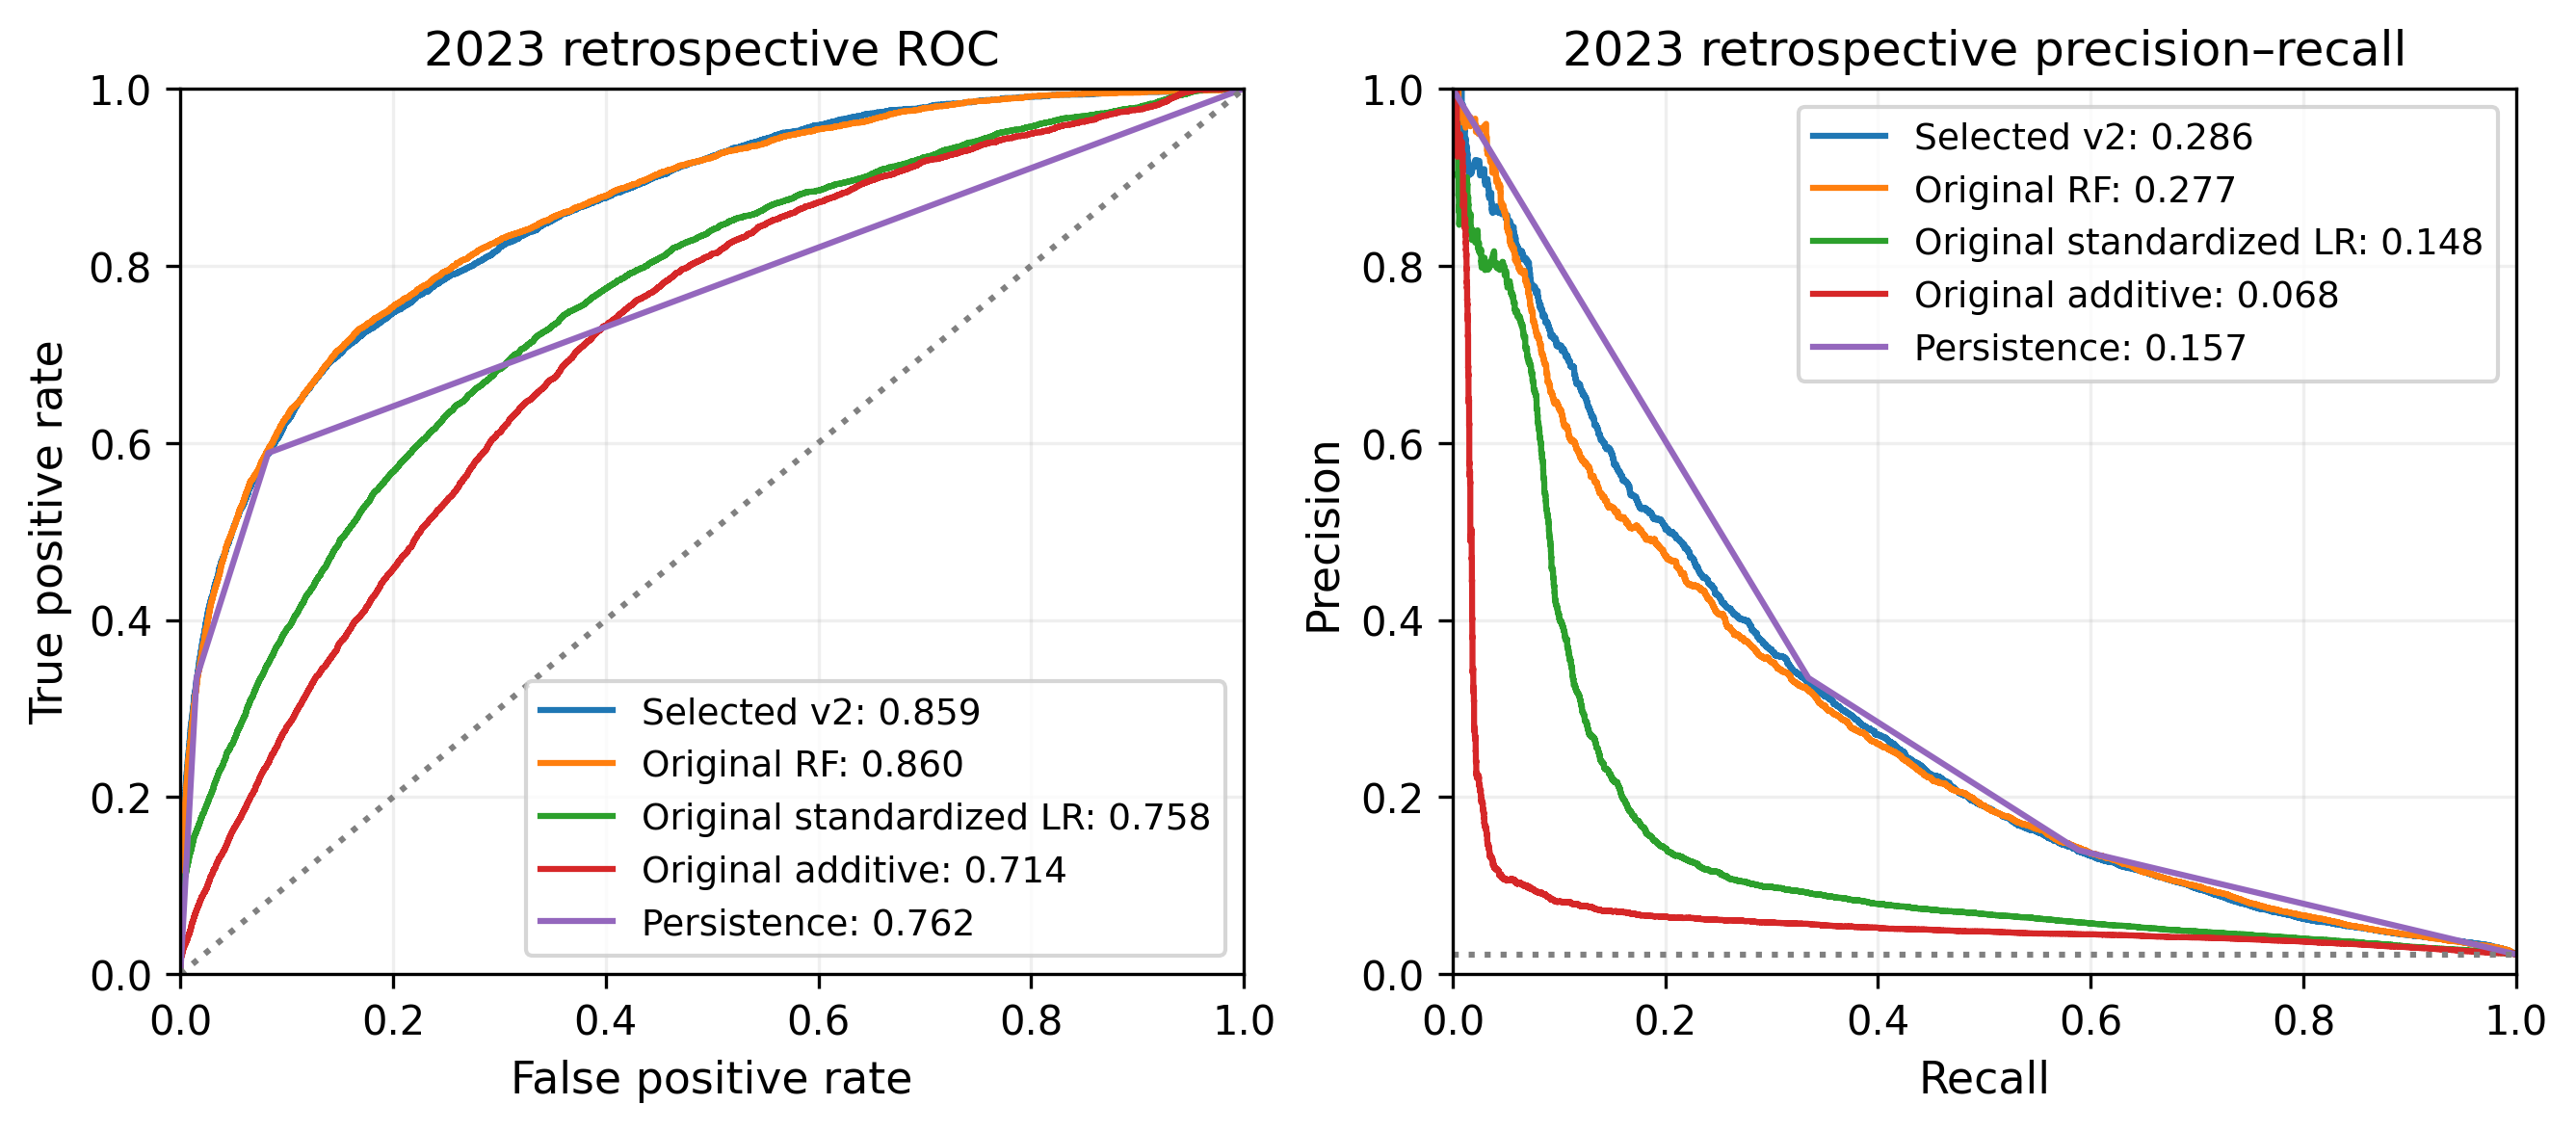
\includegraphics[width=.96\textwidth]{outputs/research/research_discrimination.png}
\caption{Retrospective benchmark ranking from saved probabilities. Legend values are AUC and AP. The dotted precision reference is the observed positive rate.}\label{fig:roc}
\end{figure*}

The comparison with the strongest original baseline is mixed. Original Random Forest scores AUC 0.8601 and AP 0.2771, whereas the selected XGBoost scores AUC 0.8592 and AP 0.2860. Its Brier score improves from 0.01876 to 0.01849, but top-decile capture falls from 60.6\% to 60.0\%. Thus the new validation rule yields better AP and probability accuracy on this benchmark without dominating every metric. A large gain over the original additive model should not be presented as an equally large gain over the strongest original ensemble.

\subsection{Matched constraints and probability behaviour}
Figure~\ref{fig:constraints} compares the sign restrictions at each fixed penalty and representation on selection data. The curves separate the effect of a coefficient bound from the effects of scaling and history compression. They should not be read as estimates of environmental causation: all fits describe conditional associations under the same satellite observation process.

\begin{figure}[!t]\centering
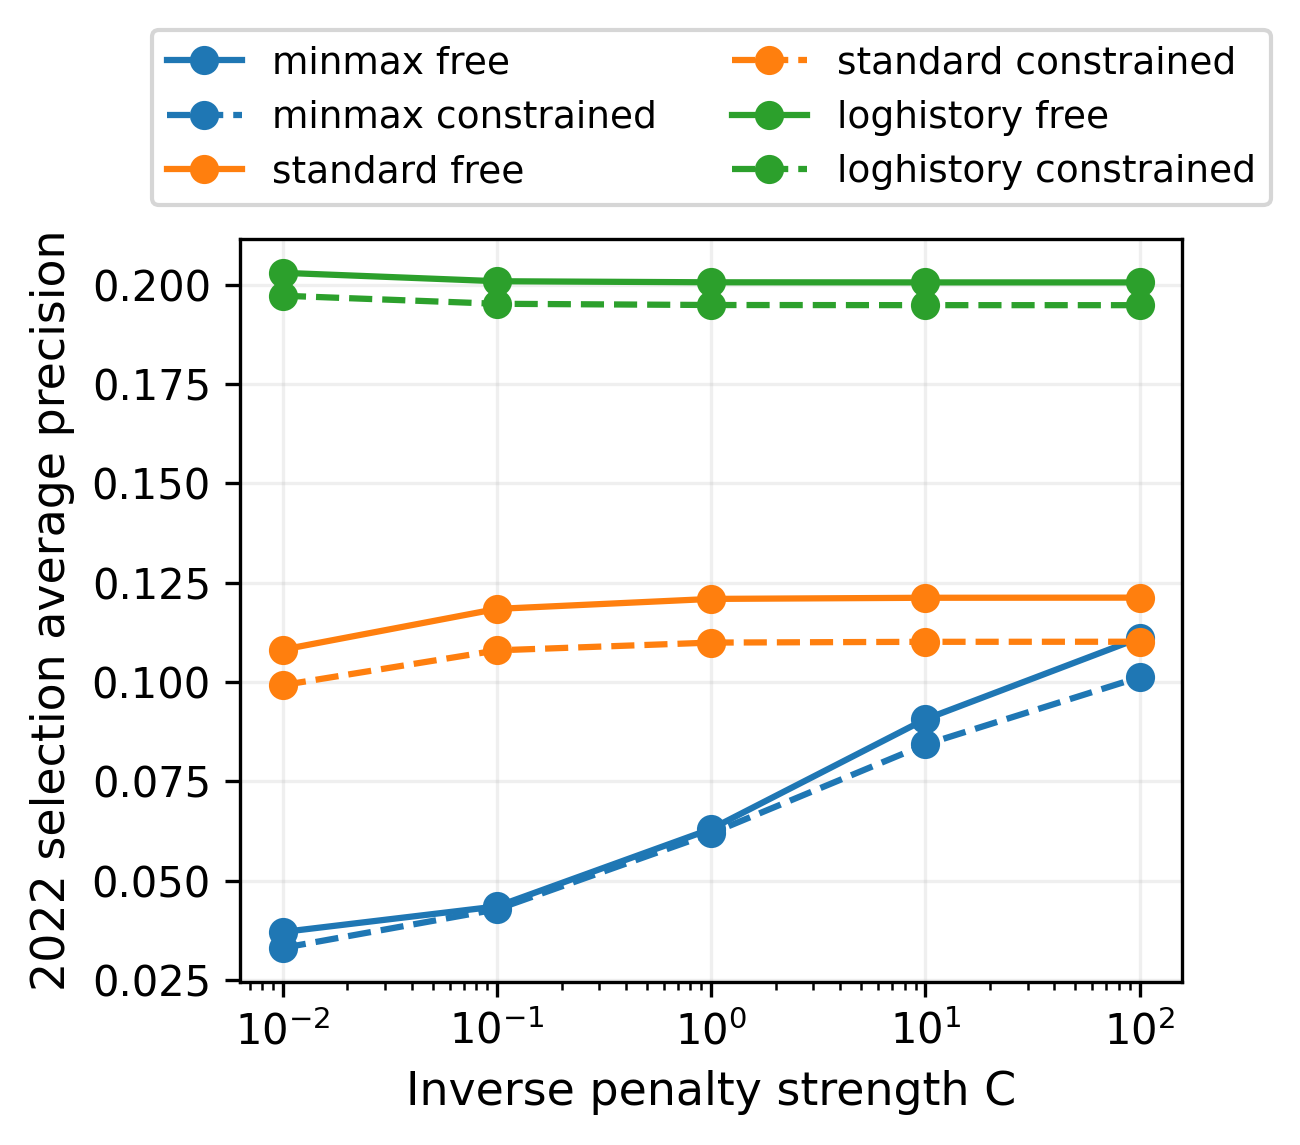
\includegraphics[width=.98\columnwidth]{outputs/research/research_constraints.png}
\caption{Matched constrained and free logistic fits on 2022 selection rows. All pairs use identical penalties, features and observations.}\label{fig:constraints}
\end{figure}

The best log-history linear fit reaches benchmark AUC 0.816 and AP 0.2370. The spline additive fit improves these to 0.839 and 0.2648, providing a useful intermediate option between a linear equation and tree ensembles. Its top-decile capture is 57.0\%. These results suggest that a flexible additive response to the existing inputs is more promising than preserving the original multiplicative gate. Within the tested offset grid, validation selects $\epsilon=0$; positive offsets do not improve the selected multiplicative formulation. This negative finding is limited to the fixed weights and offsets tested.

The new Random Forest family winner has benchmark AP 0.2919, slightly higher than the selected XGBoost's 0.2860. It is retained in Table~\ref{tab:results}, but does not replace the primary model because its selection AP is lower. Choosing it after seeing the benchmark would change the declared selection rule.

The equal-count reliability plot in Fig.~\ref{fig:reliability} describes the final mapped probabilities on 2023. Equal-count bins stabilise sample sizes but can hide within-bin errors and the behaviour of a small extreme tail. Agreement in average probability alone does not establish calibration throughout the score range. The saved raw and mapped Brier scores permit the contribution of the probability mapping to be checked separately from ranking.

\begin{figure}[!t]\centering
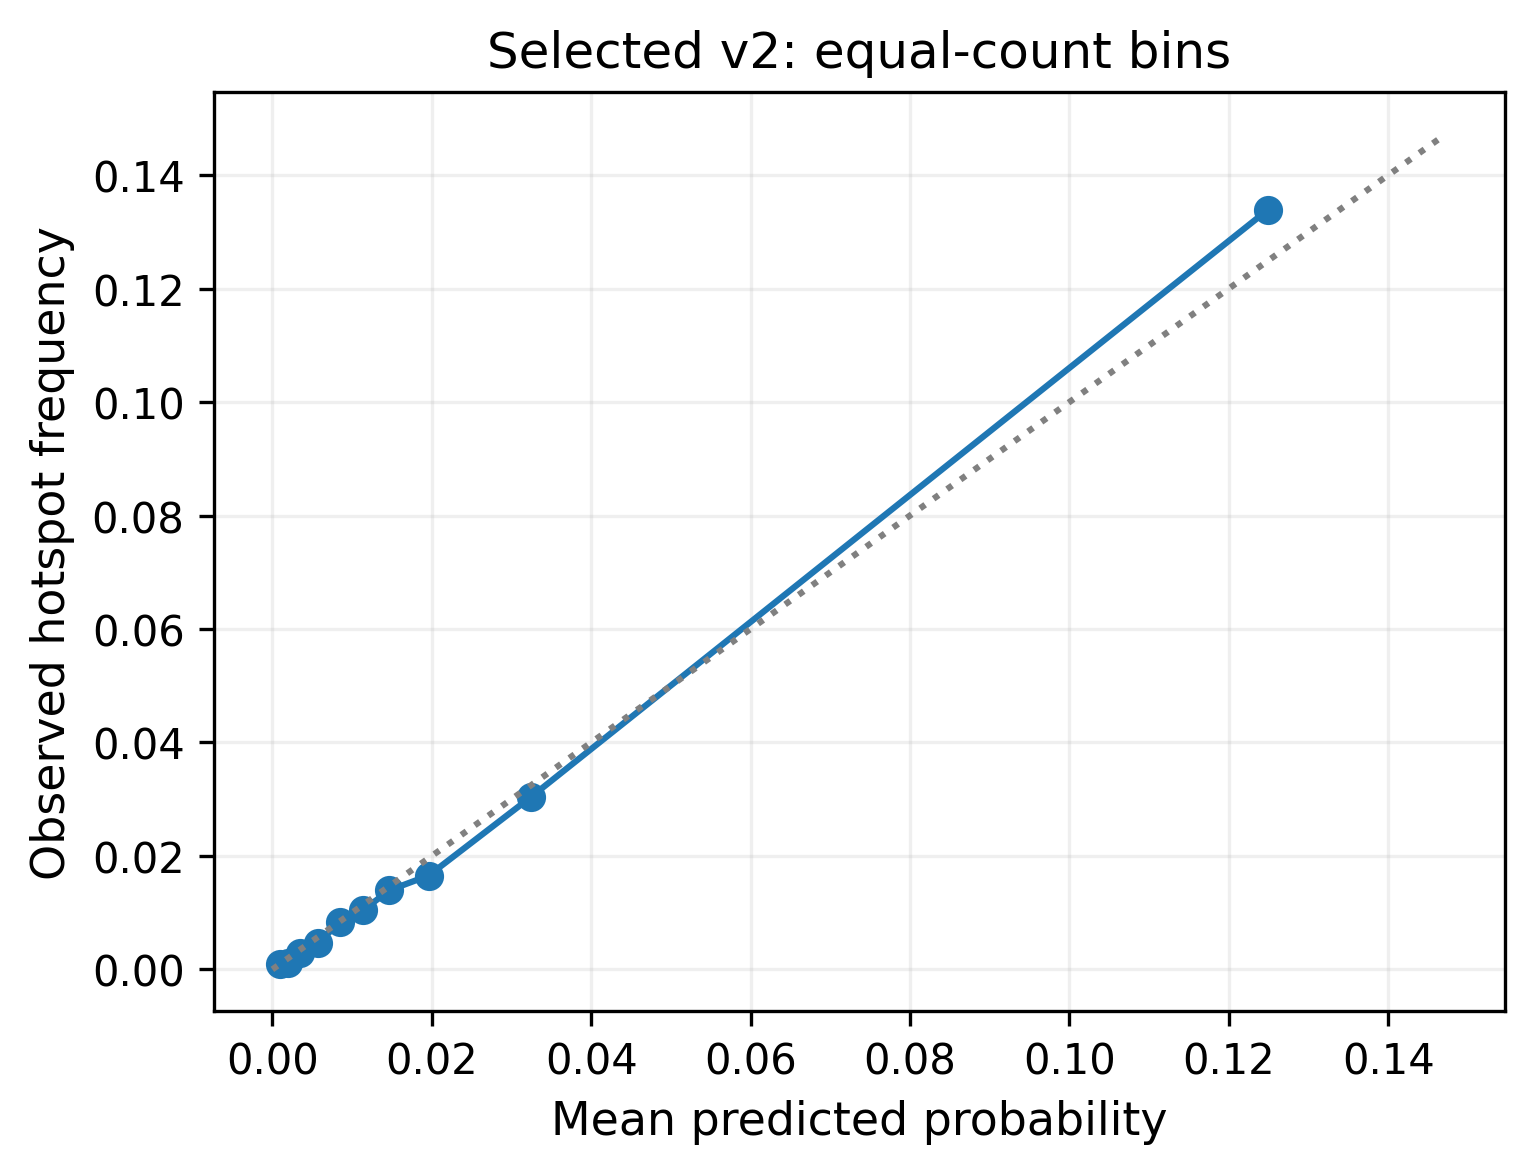
\includegraphics[width=.94\columnwidth]{outputs/research/research_reliability.png}
\caption{Selected model's final probabilities against observed 2023 frequency in ten equal-count bins. The dotted line indicates exact calibration.}\label{fig:reliability}
\end{figure}

\begin{table*}[!t]\centering\footnotesize
\caption{Selected v2 minus original comparator AUC and AP. Intervals use full-population paired moving-day blocks, 300 replicates each.}
\label{tab:bootstrap}
\begin{tabular}{rlrrrr}\toprule
Block days & Comparator & AUC difference & 95\% interval & AP difference & 95\% interval\\\midrule
7 & Original additive & +0.145 & [+0.130, +0.158] & +0.218 & [+0.188, +0.248] \\
7 & Original standardized LR & +0.101 & [+0.092, +0.109] & +0.138 & [+0.121, +0.154] \\
7 & Original RF & -0.001 & [-0.003, +0.001] & +0.009 & [+0.000, +0.016] \\
7 & Persistence & +0.097 & [+0.088, +0.109] & +0.129 & [+0.106, +0.153] \\
30 & Original additive & +0.145 & [+0.119, +0.168] & +0.218 & [+0.163, +0.260] \\
30 & Original standardized LR & +0.101 & [+0.089, +0.113] & +0.138 & [+0.115, +0.157] \\
30 & Original RF & -0.001 & [-0.004, +0.002] & +0.009 & [+0.002, +0.015] \\
30 & Persistence & +0.097 & [+0.082, +0.117] & +0.129 & [+0.091, +0.157] \\
\bottomrule\end{tabular}\end{table*}

\section{Interpretation and Limits}
\subsection{What an improvement would mean}
This search changes the statistical representation and fitting procedure, while retaining the original observation target and nine environmental/history drivers. A gain therefore shows that the preceding formulation left exploitable predictive structure in those inputs. It does not demonstrate that the new model has discovered an ignition mechanism. In particular, recent FRP and counts can identify continuation of observed activity, and the same-day weather aggregates remain retrospective.

The matched logits address a specific weakness of the preceding comparison: equal $C$ values under different scales do not imply equal penalties on equivalent physical effects. Standardizing a rare, highly concentrated history feature changes how expensive its fitted effect is under ridge regularisation. Log compression goes further by changing the response shape. The spline and interaction candidates test additional flexibility, but their larger hypothesis spaces increase the scope for fitting idiosyncrasies of one training year. A validation gain is evidence for the declared selection rule within this dataset, not a reason to dispense with later testing.

The softened multiplicative candidates retain strong restrictions. A temperature minimum is not a physical zero for fire activity, and adding an offset only partially addresses that dependence on scaling. The selected model should therefore be described by its fitted statistical form rather than as a universal physical risk equation. Even when a constrained model performs well, a positive coefficient does not prove that changing the corresponding variable would increase fire occurrence.

\subsection{Uncertainty, calibration and monitoring use}
The full-population bootstrap improves on the preceding negative-subsample analysis by retaining the actual benchmark class distribution and longer episodes. It still resamples only one year's conditions. The 7-day and 30-day intervals are sensitivity checks, not competing tests from which the narrower interval should be selected. Their uncertainty excludes the effects of changing training years, sensor coverage, grid size and hyperparameter search.

Class weighting and resampling alter the fitting distribution. Calibration on observed 2022 rows helps correct probability scale, but a new year's prevalence and conditional relationships can change. The split calibration experiment selects a mapping using a modest number of positive observations. Its assessment score is itself a selection score; the 2023 reliability diagram is consequently more informative about transport of that mapping, while still belonging to a previously examined benchmark.

For monitoring, a high AP does not specify a deployment threshold. The 10\% budget is an interpretable reference that may exceed a real team's capacity. False alarms, repeated flags for the same incident, missed fires and the costs of inspecting cells would need to be measured with an operational partner. Calibration and discrimination support that discussion, but neither is a deployment study.

\subsection{Independent evaluation and scope of optimality}
The available complete predictor archive ends in 2023. We therefore make no claim of a fresh independent test. The preceding 2023 results motivated which deficiencies to address, and this indirect reuse cannot be removed by a validation-only parameter search. A later fully acquired year, with model and threshold frozen before its labels are examined, is the next required test. Spatially held-out regions and several training years would further assess transfer and stability.

The current search covers 61 declared configurations, not all possible formulas or hyperparameters. It does not jointly optimise the multiplicative weights and offsets, combine models into an ensemble, or introduce forecast weather, incident-linked labels, or land-use information. Expanding any of those directions after inspecting the benchmark would be additional development. The reproducible candidate ledger and frozen selection artifacts make the present boundary explicit, so improvements and remaining failures can be evaluated without overstating optimality.

\section{Conclusion}
A controlled follow-up can strengthen a hotspot model by testing its statistical assumptions rather than preserving an appealing formula. The validation-selected XGBoost reaches 0.859 AUC and 0.2860 AP on the retrospective 2023 benchmark, with 60.0\% capture at a 10\% row budget. Matched regularisation, transformed histories, nonlinear alternatives and separately selected calibration make the comparison more informative than a single fitted score. The supplied candidate records, predictions and moving-block intervals support direct reproduction. Independent later-year validation remains necessary before claiming generalisation or advance ignition forecasting skill.

\section*{Acknowledgment}
The authors acknowledge Copernicus, NASA FIRMS and LP DAAC, USGS, and the US Census Bureau for the source products.
\begin{thebibliography}{00}
\bibitem{schroeder} W.~Schroeder, P.~Oliva, L.~Giglio, and I.~A.~Csiszar, ``The new VIIRS 375 m active fire detection data product,'' \emph{Remote Sensing of Environment}, vol.~143, pp.~85--96, 2014, doi:10.1016/j.rse.2013.12.008.
\bibitem{jones} M.~W.~Jones \emph{et al.}, ``State of wildfires 2023--2024,'' \emph{Earth System Science Data}, vol.~16, pp.~3601--3685, 2024, doi:10.5194/essd-16-3601-2024.
\bibitem{wooster} M.~J.~Wooster, G.~Roberts, G.~L.~W.~Perry, and Y.~J.~Kaufman, ``Retrieval of biomass combustion rates and totals from fire radiative power observations,'' \emph{Journal of Geophysical Research: Atmospheres}, vol.~110, D24311, 2005, doi:10.1029/2005JD006318.
\bibitem{era5} Copernicus Climate Change Service, ``ERA5 hourly data on single levels from 1940 to present,'' Climate Data Store, doi:10.24381/cds.adbb2d47.
\bibitem{earthmover} Earthmover, ``Icechunk ERA5: public analysis-ready reanalysis archive,'' Registry of Open Data on AWS, \url{https://registry.opendata.aws/earthmover-era5/}, accessed Nov.~2026.
\bibitem{firms} NASA FIRMS, ``VIIRS S-NPP 375 m active fire detections: Standard Processing,'' \url{https://firms.modaps.eosdis.nasa.gov/content/descriptions/FIRMS_VIIRS_Firehotspots.html}, accessed Nov.~2026.
\bibitem{modis} NASA LP DAAC, ``MOD13A2.061 MODIS/Terra Vegetation Indices 16-Day L3 Global 1 km,'' \url{https://lpdaac.usgs.gov/products/mod13a2v061/}, accessed Nov.~2026.
\bibitem{srtm} NASA LP DAAC, ``SRTM Collection User Guide,'' \url{https://lpdaac.usgs.gov/documents/179/SRTM_User_Guide_V3.pdf}, accessed Nov.~2026.
\end{thebibliography}
\end{document}